\documentclass[11pt]{article}
\usepackage[letterpaper,margin=1in]{geometry}
\usepackage{amsmath,amsbsy,amsfonts,amssymb,amsthm,commath}
\usepackage[round]{natbib}
\usepackage{hyperref}
\usepackage{graphicx}
\usepackage{float}

% math font macros

\def\ddefloop#1{\ifx\ddefloop#1\else\ddef{#1}\expandafter\ddefloop\fi}
% Blackboard fonts: \bbA, \bbB, ...
\def\ddef#1{\expandafter\def\csname bb#1\endcsname{\ensuremath{\mathbb{#1}}}}
\ddefloop ABCDEFGHIJKLMNOPQRSTUVWXYZ\ddefloop
% Calligraphic fonts: \cA, \cB, ...
\def\ddef#1{\expandafter\def\csname c#1\endcsname{\ensuremath{\mathcal{#1}}}}
\ddefloop ABCDEFGHIJKLMNOPQRSTUVWXYZ\ddefloop
% Bold fonts (for vectors, matrices, etc.): \vA, \vB, ..., \va, \vb, ...
\def\ddef#1{\expandafter\def\csname v#1\endcsname{\ensuremath{\boldsymbol{#1}}}}
\ddefloop ABCDEFGHIJKLMNOPQRSTUVWXYZabcdefghijklmnopqrstuvwxyz\ddefloop
% Bold fonts (for vectors, matrices, etc.): \valpha, \vbeta, ...,  \vGamma, \vDelta, ...,
\def\ddef#1{\expandafter\def\csname v#1\endcsname{\ensuremath{\boldsymbol{\csname #1\endcsname}}}}
\ddefloop {alpha}{beta}{gamma}{delta}{epsilon}{varepsilon}{zeta}{eta}{theta}{vartheta}{iota}{kappa}{lambda}{mu}{nu}{xi}{pi}{varpi}{rho}{varrho}{sigma}{varsigma}{tau}{upsilon}{phi}{varphi}{chi}{psi}{omega}{Gamma}{Delta}{Theta}{Lambda}{Xi}{Pi}{Sigma}{varSigma}{Upsilon}{Phi}{Psi}{Omega}{ell}\ddefloop

% other macros

\newcommand\ip[1]{\langle #1 \rangle} % inner product
\newcommand{\E}{\ensuremath{\mathbb{E}}} % expectation
\renewcommand{\P}{\ensuremath{\mathbb{P}}} % probability
\newcommand{\var}{\ensuremath{\operatorname{var}}} % variance
\newcommand{\vol}{\ensuremath{\operatorname{vol}}} % volume
\newcommand{\unitball}[1][d]{\ensuremath{B^{#1}}} % unit ball
\newcommand{\unitsphere}[1][d-1]{\ensuremath{S^{#1}}} % unit sphere
\newcommand{\logmgf}[1]{\ensuremath{\psi_{#1}}} % log mgf
\newcommand{\Normal}{\ensuremath{\operatorname{N}}} % normal distribution

% environments

\newtheorem{theorem}{Theorem}
\newtheorem{lemma}{Lemma}
\theoremstyle{definition}
\newtheorem{problem}{Problem}
\newenvironment{solution}{\noindent\emph{Solution.}}{\hfill$\square$}

%-------------------------------------------------------------------------------
% define my own command:
\newcommand\tab[1][1cm]{\hspace*{#1}}

\usepackage{listings} %For code in appendix
  \lstset{language=Java, numbers=left, showspaces=false, %Set code style
    showstringspaces=false, tabsize=2, breaklines=true}



\begin{document}

%-------------------------------------------------------------------------------
\begin{center}
\Large{} 
\textbf{CSORW4231 HOMEWORK 2} \\
\normalsize{}
Due Mon, Feb 20 \\
\large{Jun Hu \\
\textbf{(jh3846)}} \\ 
------------------------------------------------------------------------------------------------------------------
\end{center}
%-------------------------------------------------------------------------------

\begin{problem}
\large{Exercise 4.3-7 (Page 87).}
\end{problem}

\begin{solution}
\\
If set $T(n) \leq cn^{\log _3 4}$, for  substitution: $\exists \ n>0, \ c>0$, $\forall \ n>n_0$, s.t.
\begin{align*}
T(n)&=4T(\frac{n}{3}) + n \\
&\leq 4(c(\frac{n}{3})^{\log _3 4}) + n \\
&\leq cn^{\log _3 4} + n \\
&\nleq cn^{\log _3 4}
\end{align*}
Failed.\\ \\
Let $T(n) \leq c_1n^{\log _3 4} - bn$, $\exists \ n>0, \ c_1>0$, $\forall \ n>n_0$,
\begin{align*}
T(n)&=4T(\frac{n}{3}) + n \\
&\leq 4(c_1(\frac{n}{3})^{\log _3 4}) - \frac{4b}{3}n + n \\
&\leq c_1n^{\log _3 4} - \frac{4b-3}{3}n \\
&\leq c_1n^{\log _3 4} - bn
\end{align*}
Let $b \geq 3$, the assumption holds.

\end{solution}

\newpage

%-------------------------------------------------------------------------------

%-------------------------------------------------------------------------------

\begin{problem}
Exercise 4.4-4 and 4.4-5 (Page 93) and Problem 4-3. (a), (c), (e), (j) (Page 108).
\end{problem}

\begin{solution}
\begin{enumerate}
    \item[\textbf{4.4-4}]
Draw recursion tree: (Figure 1)
    \begin{figure}[htbp]
   \centering
  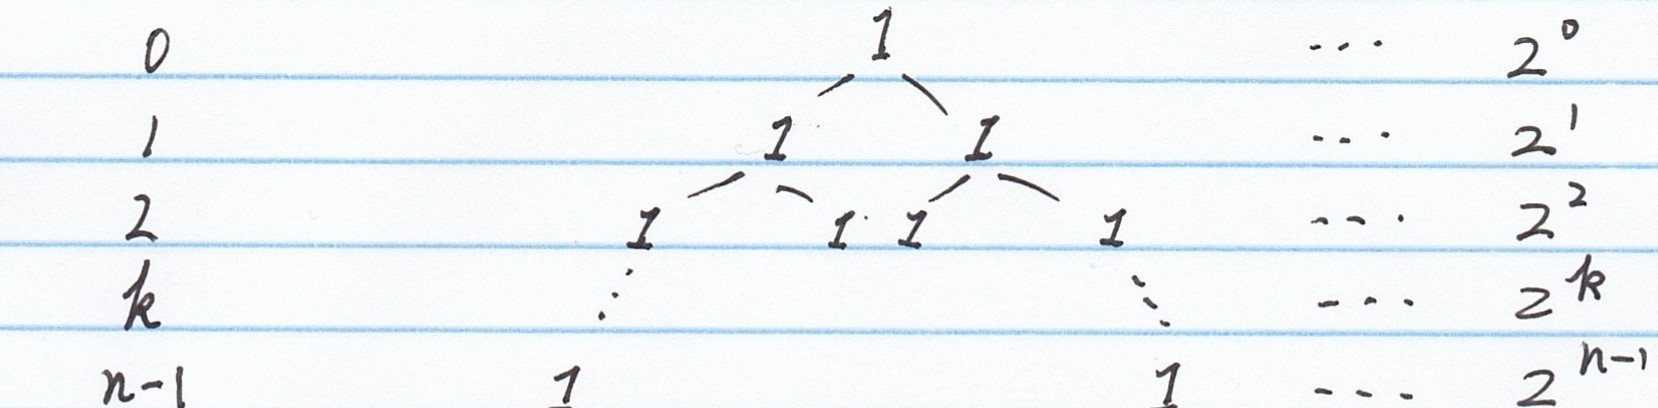
\includegraphics[width=0.8\textwidth]{/Users/vibrioh/Pictures/f1}
  \caption{Recursion Tree of 4.4-4}
  \label{fig:shapes}
\end{figure}

So $$T(n) = \sum_{k = 0}^{n - 1} 2^k = \frac{2^n-1}{2-1} = 2^n - 1 = O(2^n)$$ 
Substitution verification: Let $T(n) \leq 2^n - 1$,
$$T(n) \leq 2 \cdot (2^{n-1}-1) + 1 = 2^n - 1$$

    \item[\textbf{4.4-5}]
 Let $R(n) = T(\frac{n}{2}) + n$, rename $n = 2^m$, s.t., $S(m) = T(n) = T(2^m)$, change variables:
 \begin{align*}
S(m) &= T(n) \\
& = T(n - 1) + R(n)\\
& = T(n - 2) + R(n-1)+R(n)\\
&=R(1) + R(2) + \cdots +R(n-1)+R(n)\\
&=\sum_{i =1}^n(T(\frac{i}{2}) + i)\\
&=\sum_{i =1}^nT(\frac{i}{2}) +\frac{n(n+1)}{2}\\
&\leq nT(\frac{n}{2}) + (n+1)T(\frac{n}{2}) \tab\leftarrow\tab  (T(\frac{n}{2}) \geq T(\frac{n-1}{2}), \ T(\frac{n}{2}) \geq \frac{n}{2}) \\
&\leq 2(n+1)T(\frac{n}{2})\\
&=2(2^m+1)S(m-1)\\
&\leq 2\cdot2^{m+1}S(m-1)
\end{align*}
Let $\lg (S(m)) = Q(m)$, s.t.,
 \begin{align*}
Q(m) &\leq 2\cdot2^{m+1}S(m-1) \\
&= \lg (2\cdot2^{m+1}S(m-1)) \\
&= \lg 2+\lg 2^{m+1}+\lg (S(m-1)) \\
&= 1+m+1 +Q(m-1)\\
&=Q(m-1)+m+2
\end{align*}
Draw recursion tree: (Figure 2)
    \begin{figure}[htbp]
  \centering
  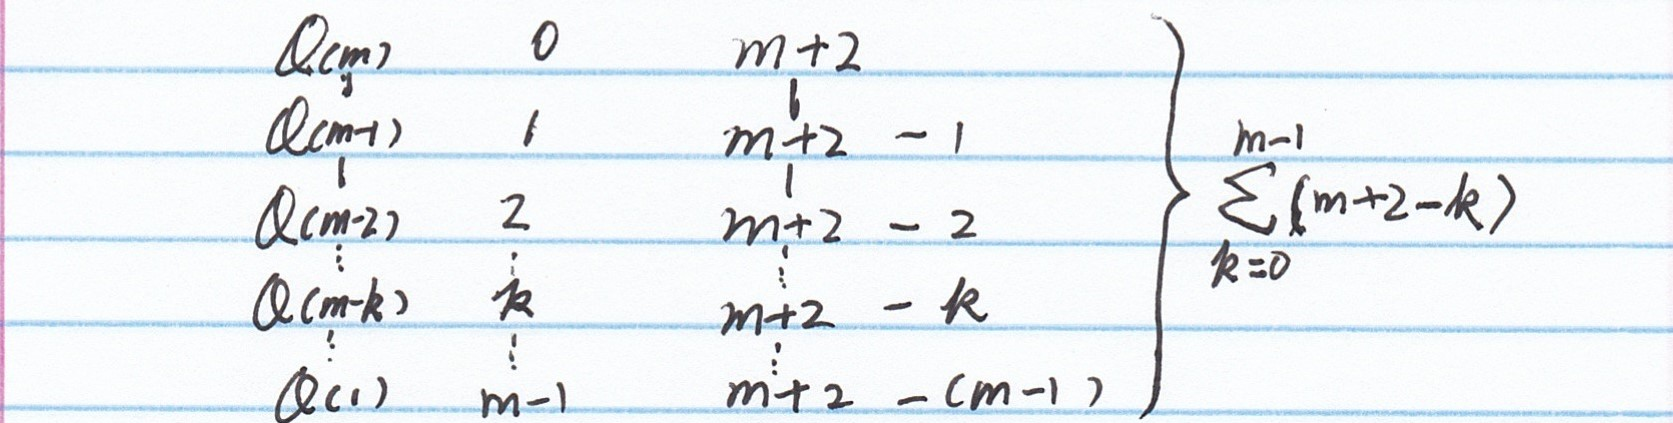
\includegraphics[width=0.8\textwidth]{/Users/vibrioh/Pictures/f2}
  \caption{Recursion Tree of 4.4-5}
  \label{fig:shapes}
\end{figure}

Guess $Q(m) = O(m^2)$, which can be verified by substitution: $\exists \  c>\frac{1}{2}$, $\forall \ m \geq \frac{c+2}{2c-1}$, s.t., $Q(m) \leq cm^2$
 \begin{align*}
Q(m) &\leq Q(m-1)+m+2\\
&=c(m-1)^2 + m + 2\\
&\leq cm^2
\end{align*}
The $S(m)$ can be calculated from $Q(m)$:
$$S(m) = O(2^{m^2})$$
Then,
$$T(n) = S(\lg n) = O(2^{\lg ^2n})$$
    
    \item[\textbf{4-3 a.}]
By Master theorem $a = 4, \ b=3, \ \epsilon > 0$, $f(n) = O(n\lg n) = O(n^{\log _34-\epsilon})$, 
\\which applies case 1:
$$T(n) = \Theta( n^{\log _34})$$

    \item[\textbf{4-3 c.}]
By Master theorem $a = 4, \ b=2, \ \epsilon > 0$, $f(n) = n^2 \sqrt{n} = \Omega( n^{2.5}) =  \Omega(n^{\log _24+\epsilon})$, \\
which applies case 3:
$$T(n) = \Theta(n^{2.5})$$

\item[\textbf{4-3 e.}]
Draw recursion tree: (Figure 3)
    \begin{figure}[htbp]
  \centering
  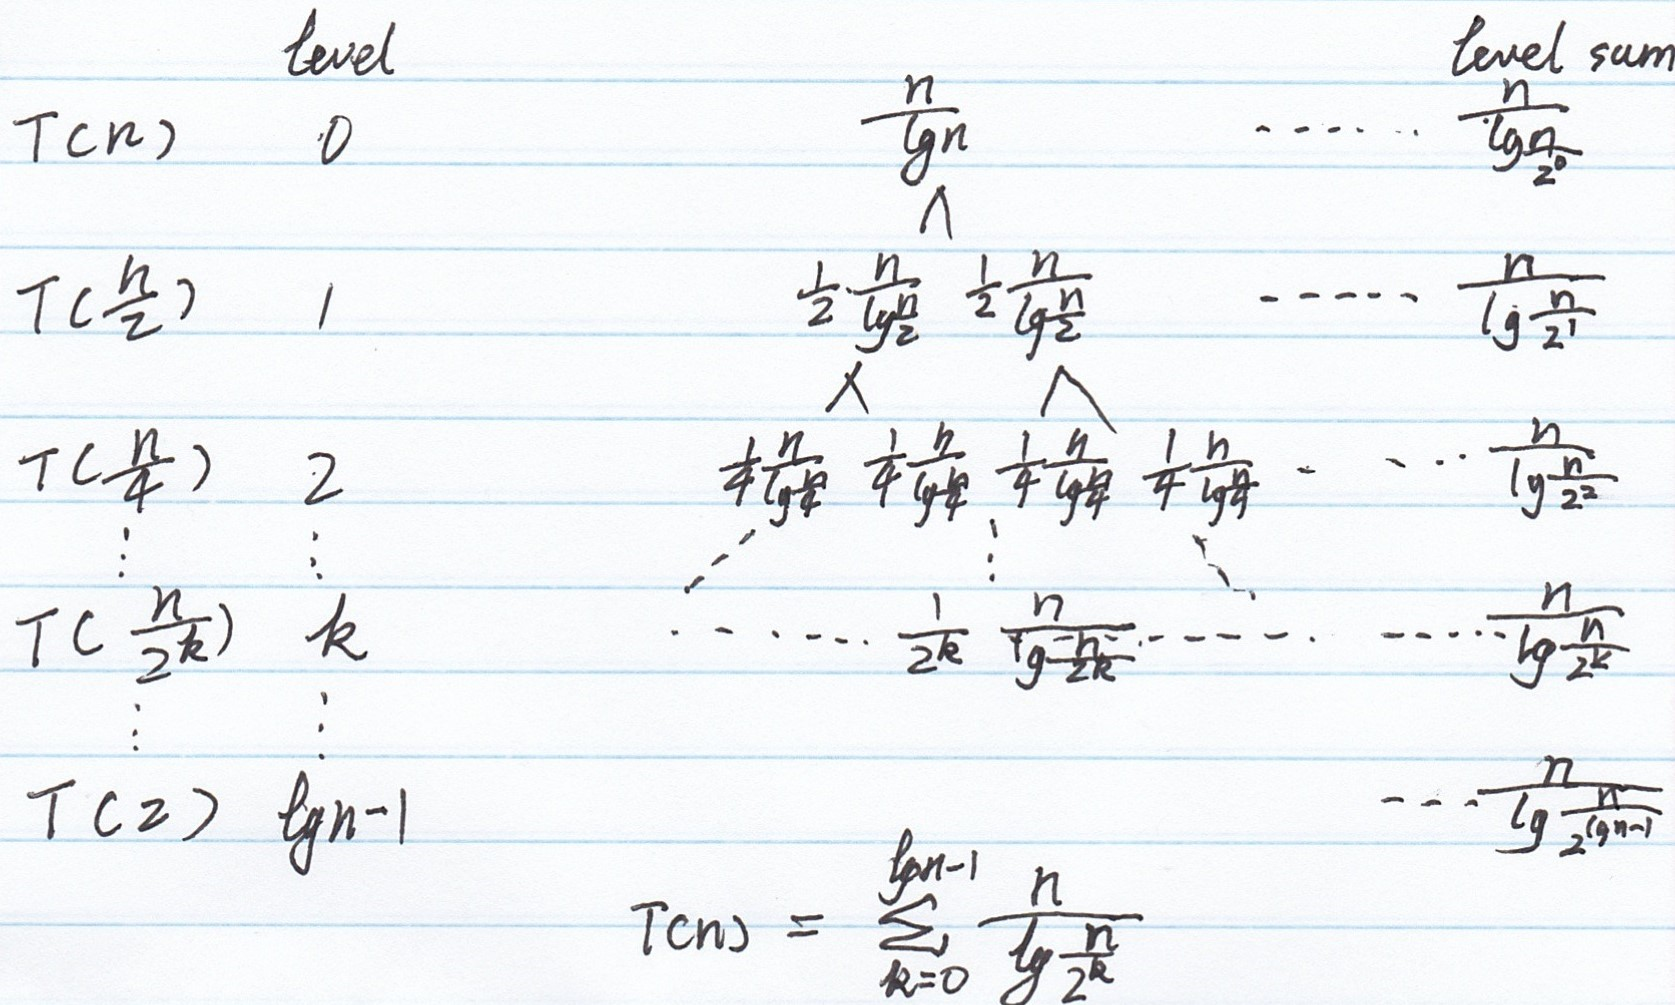
\includegraphics[width=0.8\textwidth]{/Users/vibrioh/Pictures/f3}
  \caption{Recursion Tree of 4-3 e.}
  \label{fig:shapes}
\end{figure}

Get $$T(n) = \sum_{k=0}^{\lg n-1}\frac{n}{\lg \frac{n}{2^k}} = O(n\lg \lg n) $$

\item[\textbf{4-3 j.}]
Draw recursion tree: (Figure 4)
    \begin{figure}[htbp]
  \centering
  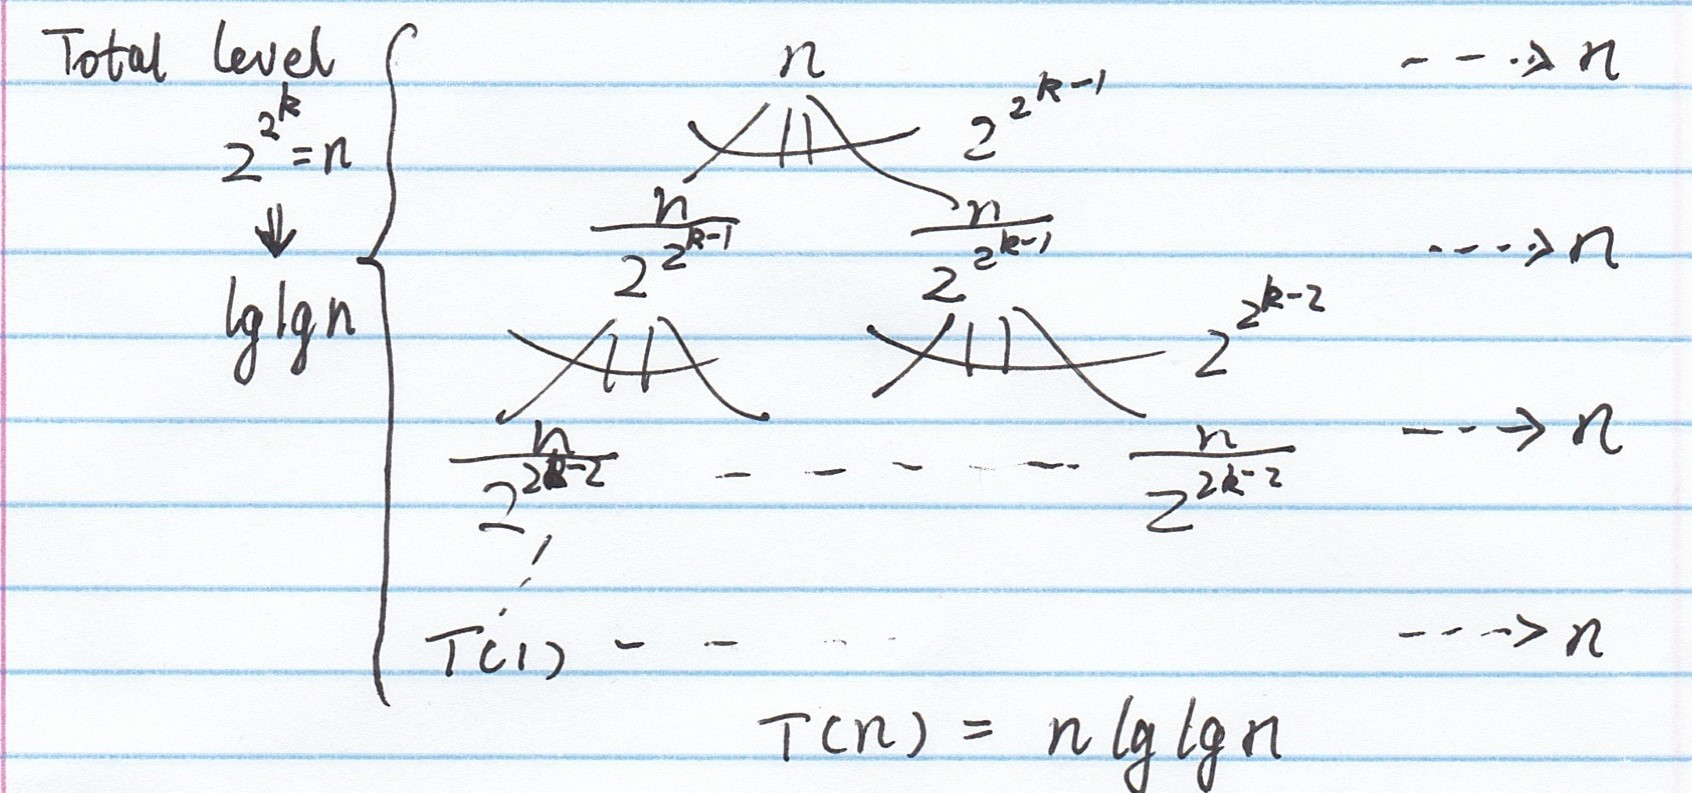
\includegraphics[width=0.8\textwidth]{/Users/vibrioh/Pictures/f4}
  \caption{Recursion Tree of 4-3 j.}
  \label{fig:shapes}
\end{figure}

So totally ($\lg \lg n $) levels, and each level has ($n$) actions, s.t., $$T(n) =  O(n\lg \lg n) $$ 
  \end{enumerate}
\end{solution}

\clearpage


%-------------------------------------------------------------------------------


%-------------------------------------------------------------------------------

%-------------------------------------------------------------------------------

\begin{problem}
Problem 4-5 (b): Chip testing.
\end{problem}

\begin{solution}
\begin{enumerate}
    \item[\textbf{Pair}]
    Pair all the chips into $ \lfloor \frac{n}{2} \rfloor $ pairs. May result in 1 unpaired chip if n is odd.

    \item[\textbf{Test}]
Test each pair.\\
    For the pairs of "both are good", remain one, discard the other one.\\
    For other pairs, discard.\\
    For the unpaired one, remain.
    


    \item[\textbf{Repeat}]
    Repeat above for the remained chips, until only one remained.\\
    The one is a good one.


\item[\textbf{Analysis}]
Among all the pairs, there are 3 combinations for chip conditions:
\begin{align*}
x &= number \ of \ \mbox{pair: "good + good"}\\
y &= number \ of \ \mbox{pair: "good + bad"} \\
z &= number \ of \ \mbox{pair: "bad + bad" }\\
\end{align*}
Except for 1 unpaired chip, if any.\\
The good chips number g(n), bad chips number b(n) s.t.,
$$
\left \{
\begin{aligned}
g(n) = 2x + y \tab\tab\tab (1)\\
b(n) = 2z + y \tab\tab\tab (2)
\end{aligned}
\right.
$$
By our algorithm, only $x + z$ 
(even) or $x + z +1$
(odd) are remained.\\
Apparently, $x +z \leq \frac{1}{2} (2x + 2y + 2z)$ (even)
or $x +z + 1 \leq \lceil\frac{1}{2} (2x + 2y + 2z + 1)\rceil$(odd) \\
Which means by $ \lfloor \frac{n}{2} \rfloor $ pairwise tests, the size of problem halved.\\
Because at the beginning of the problem, good chips are more than $\frac{n}{2}$, s.t.,\\
For even, equation $(1) - (2)$, remained $x > z$, good chips are still more than $\frac{n}{2}$ in the new problem.\\
For odd, 1 unpaired is good, $g(n)+1>b(n)$, $x+1 > z$, good chips are still more than $\frac{n}{2}$ in the new problem.\\
For odd, 1 unpaired is bad, $g(n)>b(n)+1$, $x> z +1$, good chips are still more than $\frac{n}{2}$ in the new problem.

\end{enumerate}

\end{solution}

\newpage

%-------------------------------------------------------------------------------

%-------------------------------------------------------------------------------

\begin{problem}Exercise 5.2-5 (Page 122) and Exercise 5.4-6 (Page 142): Indicator random variables.
\end{problem}

\begin{solution}
  \begin{enumerate}
  
    \item[\textbf{5.2-5}]
    For $1 \leq i \leq j \leq n$, let $X_{i,j}$ be an event of pair $i, \ j$, as an inversion of array $A$,
    $$X_{i,j}=
\left \{
\begin{aligned}
1,\  A[i] > A[j]\\
0, \ A[i]< A[j]
\end{aligned}
\right.
$$
Calculate the expectation of total number of inversions $X$
\begin{align*}
E \left[  X \right] &= E \left[ \sum_{i,j}X_{i,j} \right] \\
& = \sum_{i,j} E \left[ X_{i,j} \right] \\
& = \sum_{i,j} Pr \{ X_{i,j} =1 \} \\
& = \sum_{i,j} \frac{1}{2} \\
&= \frac{1}{2} \sum_{i=1}^{n-1}\sum_{j=i+1}^n1\\
&= \frac{1}{2} \sum_{i=1}^{n-1} \left(n-i \right) \\
&=  \frac{1}{2}  \left(  n(n-1) -   \frac{n(n-1)}{2}    \right) \\
&= \frac{n(n-1)}{4}
\end{align*}

   \item[\textbf{5.4-6}]
Let $X_i$ be an event of blank bin after n times tosses, $Y_j$ be an event of a bin with exactly one ball after n times tosses., s.t.,
\begin{align*}
Pr \{ X_i = 1  \} &= \left(  1- \frac{1}{n}   \right) ^n \\
Pr \{ Y_j = 1  \} &= \frac{1}{n} { n \choose 1   } \left(  1- \frac{1}{n}   \right) ^{n-1} =\left(  1- \frac{1}{n}   \right) ^{n-1}
\end{align*}
For the event numbers $X$, $Y$, the expectations are:
\begin{align*}
E \left[  X \right] &= E \left[ \sum_{i=1}^n X_i \right] \\
&=  \sum_{i=1}^n E \left[ X_i \right] \\
&= \sum_{i=1}^n  Pr \{  X_i = 1   \} \\
&= \sum_{i=1}^n \left(  1- \frac{1}{n}   \right) ^n \\
&= n \left(  \frac{n-1}{n}   \right) ^n
\end{align*}
\begin{align*}
E \left[  Y \right] &= E \left[ \sum_{i=1}^n Y_j \right] \\
&=  \sum_{j=1}^n E \left[ Y_j \right] \\
&= \sum_{j=1}^n  Pr \{  Y_j = 1   \} \\
&= \sum_{j=1}^n \left(  1- \frac{1}{n}   \right) ^{n-1} \\
&= n \left(  \frac{n-1}{n}   \right) ^{n-1}
\end{align*}

    
    
  \end{enumerate}
\end{solution}

\newpage
%-------------------------------------------------------------------------------

%-------------------------------------------------------------------------------

%-------------------------------------------------------------------------------

\begin{problem}
Problem 7-3 (Page 187): Alternative quicksort analysis.
\end{problem}

\begin{solution}
\begin{enumerate}
   \item[\textbf{a.}]
   Pivot is randomly picked from $n$ length array, so the probability is $\frac{1}{n}$, s.t.,
   $$
   E \left[  X_i \right] = Pr \{ X_i = 1  \} = \frac{1}{n}
   $$
   
      \item[\textbf{b.}]
If the pivot is at $q$, then the array will be separated as subarrays with the size of $q-1$ and $n-q$. And this action of partition takes $O(n)$. This is how $ E \left[  T(n) \right]$ comes to be.

     \item[\textbf{c.}]
     Rewrite the equation with explanations:
     \begin{align*}
     E \left[  T(n) \right] &=  E \left[    \sum_{q=1}^n X_q \left(  T(q-1) + T(n-q) + \Theta(n)    \right)  \right] \\
     &=    \sum_{q=1}^n E \left[   X_q \left(  T(q-1) + T(n-q) + \Theta(n) \right) \right] \tab\leftarrow\tab \mbox{linearity of expectation}\\
     &=   \sum_{q=1}^n E \left[   X_q \right] \cdot E \left[  \left(  T(q-1) + T(n-q) + \Theta(n) \right) \right] \tab\leftarrow\tab \mbox{$X_q$ independence}   \\
     &=     \sum_{q=1}^n E \left[   X_q \right] \cdot \left(  E  \left[   T(q-1)\right] + E \left[ T(n-q) \right] + E \left[ \Theta(n) \right]   \right)  \\
          &=  \sum_{q=1}^n \frac{1}{n}  \left(  E  \left[   T(q-1)\right] + E \left[ T(n-q) \right] + E \left[ \Theta(n) \right]   \right) \tab\leftarrow\tab \mbox{from \textbf{a.}}  \\    
     &=  \frac{1}{n} \left( \sum_{q=1}^n     E  \left[   T(q-1)\right] + \sum_{q=1}^n E \left[ T(n-q) \right] + \sum_{q=1}^n E \left[ \Theta(n) \right]   \right)         \\
     &=  \frac{1}{n} \left( \sum_{q=0}^{n-1}     E  \left[   T(q)\right] + \sum_{q=0}^{n-1} E \left[ T(q) \right] + n  \Theta(n)   \right)  \tab\leftarrow\tab q' =(q-1)\ \mbox{or} \ (n - q) \\
     &=  \frac{2}{n} \sum_{q=2}^{n-1}     E  \left[   T(q)\right] +\frac{2}{n} \left( E  \left[   T(0)\right] +E  \left[   T(1)\right] \right)   + \Theta(n)  \\
  &=   \frac{2}{n} \sum_{q=2}^{n-1}     E  \left[   T(q)\right]  + \Theta(n)  \tab\leftarrow\tab T(0)=T(1)=\Theta(1) 
     \end{align*}

     \item[\textbf{d.}]
     Proof
     \begin{align*}
\sum_{k=2}^{n-1} k \lg k
&= \sum_{k=2}^{\lceil \frac{n}{2} \rceil -1} k \lg k + \sum_{k=\lceil \frac{n}{2} \rceil}^{n-1} k \lg k \\
&\leq \sum_{k=2}^{\lceil \frac{n}{2} \rceil -1} k \lg \frac{n}{2} + \sum_{k=\lceil \frac{n}{2} \rceil}^{n-1} k \lg n \\
&= \lg \frac{n}{2}  \sum_{k=2}^{\lceil \frac{n}{2} \rceil -1} k + \lg n \sum_{k=\lceil \frac{n}{2} \rceil}^{n-1} k  \\
&= \lg \frac{n}{2} \left(  \frac{\frac{n}{2}(\frac{n}{2}-1)}{2}  \right) +  \lg n \left( \frac{n(n-1)}{2} - \frac{\frac{n}{2}(\frac{n}{2}-1)}{2}  \right) \\
&\leq \left( \lg \frac{n}{2} \right) \cdot \frac{n^2}{8} + \left( \lg n \right) \left( \frac{n^2}{2} - \frac{n^2}{8} \right)  \\
&= \frac{1}{2} n^2 \lg n - \frac{1}{8} n^2
     \end{align*}
     
      \item[\textbf{e.}]
    
    Guess $E  \left[   T(q)\right] \leq cq \lg q $, $\forall \ 2 \leq q<n, \ a>0, c>0, n_0>0$, s.t.,
     \begin{align*}
     E \left[  T(n) \right] &=  \frac{2}{n} \sum_{q=2}^{n-1}     E  \left[   T(q)\right]  + \Theta(n) \\
     &\leq \frac{2}{n} \sum_{q=2}^{n-1}     cq \lg q  + an \\
     &= \frac{2}{n} c \left( \frac{1}{2} n^2 \lg n - \frac{1}{8} n^2 \right) + an \\
     &= cn \lg n - \left(      \frac{c}{4}  -a       \right)n \\
     &\leq cn \lg n \tab\Leftarrow\tab \forall \ n>n_0, \ \exists \ c \geq 4a \\
     \end{align*}


\end{enumerate}



\end{solution}




\end{document}